\part{Nivel de Red}
\begin{figure}[H]
	\centering
	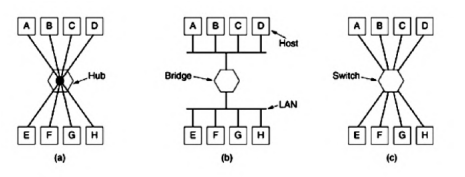
\includegraphics[width=\textwidth
]{images/topologias-red.png}
	\caption[Topologías de Red]{Topologías de Red}
	\label{fig:topologias-red}
\end{figure}
En la figura \ref{fig:topologias-red} se pueden ver tres tipos de LAN:
\begin{enumerate}[a)]
  \item En la primera vemos un conjunto de hosts conectados por un \textbf{hub}, esto es: Todos los hosts están conectado
  s entre sí como si los uniese un único cable. El \textbf{hub}, como los \textbf{repetidores} (amplificadores de señal), funcionan a nivel físico permitiendo agregar equipos a una red.
  \item En el segundo, un puente o \textbf{bridge}, separa en dos grupos los hosts de la red creando dos zonas independientes para la detección de colisiones. En este caso los hosts de un grupo podrán emitir sin tener que preocuparse por interferir con los hosts del otro grupo. Un paquete enviado la dirección de \textbf{broadcast}, alcanza a todos los hosts de la LAN.
  
  Puede interconectar, dos tipos de tecnología distintas (por ejemplo, ethernet y wifi). Por esta razón en la capa MAC, se agrega al header del paquete un campo que permite identificar el tipo de red del que viene. Cuando el bridge capta el paquete y se da cuenta que el host está en una red de distinto tipo, cambia el header para que matcheen y lo reenvía a través de la tecnología correspondiente
  \item Por último tenemos un conjunto de host conectados por un \textbf{switch}: Cada host se conecta con una conexión full-duplex al dispositivo, que se encarga de recibir todos los mensajes de un host y redireccionarlo al host correspondiente. En este tipo de redes se elimina la necesidad detectar colisiones y se pasa a necesitar un algoritmo que permita al switch realizar el dispatch de los mensajes de manera correcta.
  
  Tanto el switch como el bridge funciona a nivel capa de enlace. Se encargan de redireccionar los frames enviados a través de una LAN para que lleguen al dispositivo correspondiente.
\end{enumerate}

Agregamos un último dispositivo: El \textbf{router}, para conectar distintas redes a nivel red. Se encargán de buscar el camino que debe seguir para llegar a destino. Cuando una host envía decide enviar un paquete, lo encapsula en un frame que contiene el tipo de protocolo usado. Cuando el paquete llega el router, este se encarga de tomar el frame que le llego, desencapsular el paquete y guardarlo en un frame adecuado para que pueda ser interpretado por los dispositivos de la nueva ren en la que ingresa el frame.

\section{Switches}
En términos simples, un switch es un mecanismo que nos permite interconectar enlaces para formar una red más grande. Un switch es un dispositivo de múltiples entradas y salidas que transfiere paquetes desde una entrada a una o más salidas. El trabajo principal de un switch es recibir paquetes entrantes en uno de sus enlaces y transmitirlos en otro enlace. Esta función se denomina a veces conmutación (\textbf{switching}) o reenvío (\textbf{forwarding}).

Por lo tanto, un switch agrega la topología de estrella a la topología de enlace punto a punto. Una topología de estrella tiene varias propiedades atractivas:

\begin{itemize}
  \item Aunque un switch tiene un número fijo de entradas y salidas, lo que limita la cantidad de hosts que se pueden conectar a un solo switch, se pueden construir redes grandes interconectando varios switches.
  \item Podemos conectar switches entre sí y a hosts usando enlaces punto a punto, lo que típicamente significa que podemos construir redes de gran alcance geográfico.
  \item Agregar un nuevo host a la red conectándolo a un switch no necesariamente reduce el rendimiento de la red para otros hosts ya conectados.
\end{itemize}

Cada host en una red conmutada (Switched network) tiene su propio enlace al switch, por lo que puede ser completamente
posible que muchos hosts transmitan a la velocidad de enlace completa (ancho de banda),
siempre que el switch esté diseñado con suficiente capacidad agregada.

En general, las redes conmutadas son consideradas más escalables. 

Cuando un router recibe un paquete, busca, en el header del paquete, un identificador que usa para decidir a que puerto. Los detalles de como usa este identificador varían, pero hay dos enfoques comunes. El primero es el enfoque \textbf{datagrama} o \textbf{sin conexión}. El segundo es el enfoque de \textbf{circuito virtual} o \textbf{orientado a conexión}. Un tercer enfoque, el \textbf{enrutamiento de origen} (\textbf{source routing}), es menos común que estos otros dos, pero tiene algunas aplicaciones útiles.

Una cosa que es común a todas las redes es que necesitamos tener una forma de identificar los nodos con los que podremos comunicardos. En general, el identificador que se les asigna se llaman \textbf{direcciones}.

Otra cosa que debemos definir es como el router va a tomar la decisión de a que puerto enviar el paquete. Para esto, se define una \textbf{tabla de enrutamiento} que asocia una dirección de destino con un puerto de salida. En general, la tabla de enrutamiento se construye a partir de un algoritmo de enrutamiento.

\subsection{Redes de datagramas}
La idea detrás de los datagramas es increíblemente simple: Incluir en cada paquete suficiente información para permitir que cualquier switch decida cómo llevarlo a su destino. Es decir, cada paquete contiene la dirección de destino completa. Para decidir cómo reenviar un paquete, un switch consulta una tabla de forwarding (a veces llamada tabla de enrutamiento).

Las redes de datagramas tienen las siguientes características:
\begin{itemize}
  \item Un host puede enviar un paquete a cualquier destino en cualquier momento, ya que cualquier paquete que llegue a un switch puede ser reenviado inmediatamente (suponiendo una tabla de forwarding correctamente poblada). Por esta razón, las redes de datagramas a menudo se llaman sin conexión; esto contrasta con las redes orientadas a conexión en las que se debe establecer algún estado de conexión antes de que se envíe el primer paquete de datos.
  \item Cuando un host envía un paquete, no tiene forma de saber si la red es capaz de entregarlo o si el host de destino incluso está activo.
  \item Cada paquete se reenvía independientemente de los paquetes anteriores que podrían haberse enviado al mismo destino. Por lo tanto, dos paquetes sucesivos de host A a host B pueden seguir rutas completamente diferentes (quizás debido a un cambio en la tabla de forwarding en algún switch de la red).
  \item Una falla de switch o enlace puede no tener ningún efecto serio en la comunicación si es posible encontrar una ruta alternativa alrededor de la falla y actualizar la tabla de forwarding en consecuencia.
 \end{itemize}

\subsection{Circuitos virtuales}
Una segunda técnica para el conmutación de paquetes, que difiere significativamente del modelo de datagrama, usa el concepto de un \textbf{circuito virtual (VC)}.

Este enfoque, que también se conoce como \textbf{modelo orientado a conexión}, requiere configurar una conexión virtual desde el host de origen hasta el host de destino antes de que se envíe cualquier dato. Podemos pensar en esto como un proceso de dos etapas. La primera etapa es la "configuración de la conexión". El segundo es la transferencia de datos.

Durante el setup de la conexión, se establece un estado de conexión en cada uno de los switches entre los hosts de origen y destino. Una sola conexión consiste en una entrada en la "tabla VC" de cada switch que describe la conexión y que interfaces dentro de ese switch están involucradas en la misma. Entonces cada entrada de la tabla VC está formada por cuatro campos:

\begin{itemize}
  \item Un \textbf{identificador de circuito virtual (VCI)} que identifica de forma única la conexión en este switch y que se llevará dentro de la cabecera de los paquetes que pertenecen a esta conexión
  \item Una \textbf{interfaz de entrada} en la que el switch va a recibir los paquetes para este VC.
  \item Una \textbf{interfaz de salida} que se usará para reenviar los paquetes asociados al VC.
  \item El \textbf{VCI de salida} que se utilizará en el nuevo header de los paquetes que se forwardean.
 \end{itemize}
 
 La semántica de estas entradas es la siguiente: Si un paquete llega a la interfaz de entrada designada y ese paquete contiene el valor VCI designado en su encabezado, entonces ese paquete debe enviarse a la interfaz de salida especificada con el valor VCI de salida especificado (se remplaza el VCI de entrada en el header del paquete recibido por el nuevo antes de forwardearlo).

 La combinación del VCI de los paquetes a medida que se reciben en el switch y la interfaz de entrada identifican de forma única la conexión virtual. Puede haber muchas conexiones virtuales establecidas en un mismo switch al mismo tiempo. Además, los valores de VCI de entrada y salida generalmente no son los mismos. Por lo que el VCI no es un identificador de importancia global para la conexión; más bien, tiene importancia solo en un enlace dado.

 Cada vez que se crea una nueva conexión, debemos asignar un nuevo VCI para esa conexión en cada enlace que la conexión atravesará. También debemos asegurarnos de que el VCI elegido en un enlace determinado no esté actualmente en uso en ese enlace por alguna conexión existente.

\subsubsection{Creación de la conexión}
 Hay dos enfoques generales para establecer el estado de conexión: Uno es que un administrador de red configure el estado, en cuyo caso el circuito virtual es "permanente" (\textbf{Permanent Virtual Cirtcuit}). Este circuito también puede ser eliminado por el administrador. Alternativamente, un host puede enviar mensajes a la red para hacer que se establezca el estado. Esto se conoce como \textbf{señalización (signaling)}, y los circuitos virtuales resultantes se denominan conmutados (switched). La característica más importante de un \textbf{circuito virtual conmutado (SVC)} es que un host puede configurarlo y eliminarlo dinámicamente sin la participación de un administrador de red.

 Suponiendo que todos los nodos de la red saben la topología y la ubicación de cada nodo (esto se hace corriendo algoritmos de routing que vamos a ver más adelante), el algoritmo para crear una conexión es el siguiente: Si el host \(A\) quiere conectarse con el host \(B\) entonces:

 \begin{enumerate}
  \item \(A\) envía un paquete con un pedido de conexión a la red que contiene la dirección completa de \(B\).
  \item El paquete llega a un switch \(S_1\) que crea una entrada en su tabla de VC para la conexión registrando la interfaz desde la que le llegó el paquete y asignando el VCI de entrada. Luego busca en su tabla de forwarding cual es el próximo nodo que debe recibir el paquete.
  \item Cada switch al que le llega el paquete realiza la misma operación hasta que el mismo llega a \(B\).
  \item Finalmente, el pedido de conexión llega a \(B\) que decide si aceptar o no la conexion. Si lo hace, también asigna un valor VCI de entrada en su tabla de VC.
  \item Para completar, la conexión \(B\) envría un mensaje de aceptación que debe recorrer el camino establecido hasta \(A\) indicando a cada uno de los nodos cual es el VCI de salida que deben usar en cada paso.
  \item Cuando el último paquete llega a \(A\), cada switch tiene una entrada completa en su tabla de VC para la conexión.
  \end{enumerate}

Cuando el \(A\) ya no quiere enviar datos a \(B\), destruye la conexión enviando un mensaje de destrucción a \(S_1\). El switch elimina la entrada relevante de su tabla y reenvía el mensaje a los otros switches en el camino, que eliminan de manera similar las entradas apropiadas de sus tablas.

Hay varias cosas a tener en cuenta sobre el conmutación de circuitos virtuales:
\begin{itemize}
  \item \(A\) tiene que esperar a que la solicitud de conexión llegue al otro lado de la red y regrese antes de que pueda enviar su primer paquete de datos, hay al menos un tiempo de ida y vuelta (RTT) de retraso antes de que esto pueda suceder.
  \item Si bien la solicitud de conexión contiene la dirección completa del \(B\) (que puede ser bastante grande, ya que es un identificador global en la red), cada paquete de datos contiene solo un identificador pequeño, que es único solo en un enlace. Por lo tanto, la sobrecarga por paquete causada por el encabezado se reduce en relación con el modelo de datagrama.
  \item Si un switch o un enlace en una conexión falla, la conexión se rompe y se deberá establecer una nueva. Además, el circuito virtual roto debe ser desmantelado para liberar espacio de almacenamiento de tablas de los switches.
\end{itemize}

\subsubsection{Comparación con el modelo de datagrama}

Una de las ventajas de los circuitos virtuales es que para cuando el host recibe la señal de que puede enviar datos, sabe bastante sobre la red, por ejemplo, que realmente hay una ruta hacia el receptor y que el receptor está dispuesto y es capaz de recibir datos. También es posible asignar recursos al circuito virtual en el momento en que se establece.

En comparación, una red de datagramas no tiene una fase de establecimiento de conexión, y cada switch procesa cada paquete de forma independiente, lo que hace menos obvio cómo una red de datagramas asignaría recursos de manera significativa. En cambio, cada paquete que llega compite con todos los demás por el espacio del búfer. Si no hay búferes libres, el paquete entrante debe descartarse.

\subsection{Source Routing}
Un tercer enfoque al switching que no utiliza ni circuitos virtuales ni datagramas convencionales se conoce como \textbf{source routing}. En esta técnica,toda la información sobre la topología de la red que se requiere para conmutar un paquete es proporcionada por el host de origen. 

Es decir, el host de origen envía un paquete con un header que contiene toda la información necesaria para forwardear el paquete a su destino. El switch simplemente lee el header y lo reenvía al siguiente nodo. Una forma de hacer esto sería poner una lista ordenada de puertos de switch por el que se debe forwardear el paquete y rotar la lista para que el siguiente switch en el camino siempre esté al frente de la lista.

Hay varias cosas a tener en cuenta sobre este enfoque:

\begin{itemize}
  \item Asume que el host de origen sabe lo suficiente sobre la topología de la red para formar un encabezado que tenga todas las direcciones correctas para cada switch en el camino.
  \item  No podemos predecir cuán grande debe ser el encabezado, ya que debe poder contener una palabra de información para cada switch en el camino. Esto implica que probablemente sean de longitud variable sin límite superior, a menos que podamos predecir con absoluta certeza el número máximo de switches a través de los cuales un paquete necesitará pasar.
  \item Hay algunas variaciones en este enfoque. Por ejemplo, en lugar de rotar el encabezado, cada switch podría simplemente eliminar el primer elemento a medida que lo usa. La rotación tiene una ventaja sobre el stripping, sin embargo: el host B obtiene una copia del encabezado completo, lo que puede ayudarlo a descubrir cómo volver al host A. Otra alternativa es que el encabezado lleve un puntero al "próximo puerto" que debe ser usado, de modo que cada switch simplemente actualice el puntero en lugar de rotar el encabezado; esto puede ser más eficiente de implementar.
\end{itemize}

El source routing se puede usar tanto en redes de datagramas como en redes de circuitos virtuales. Por ejemplo, el Protocolo de Internet (IP), que es un protocolo de datagramas, incluye una opción de source routing que permite que se enrutan los paquetes seleccionados, mientras que la mayoría se conmutan como datagramas convencionales.

\subsection{Bridges and LAN Switches}
Comenzamos considerando una clase de switch que se usa para reenviar paquetes entre LAN (redes de área local) como Ethernets. Dichos switches a veces se conocen con el nombre obvio de \textbf{LAN switches}; históricamente, también se los ha denominado \textbf{bridges}, y se usan ampliamente en redes de campus y empresas.

Este tipo de nodo implementan completamente la detección de colisiones y los protocolos de acceso al medio en cada una de sus interfaces. Por lo tanto, las restricciones del protocolo sobre la distancia y número de hosts no se aplicarían al par de redes combinadas de esta manera. Este dispositivo opera en modo promiscuo, aceptando todos los tramas transmitidos en cualquiera de las redes y reenviándolos al otro.

Una colección de redes conectadas por uno o más bridges se dice que forman una \textbf{LAN extendida}.

\subsubsection{Learning Bridges}
La primera optimización que podemos hacer a un bridge es observar que no necesita reenviar todos los frames que recibe.

Para esto podemos hacer que cada bridge inspeccione la dirección de origen de todos los frames que recibe. Cuando un host \(A\) envía un frame a otro cualquiera, el bridge recibe este frame y registra el hecho de que se acaba de recibir un frame de \(A\) en tal interfaz \(I\). De esta manera, cuando reciba un mensaje que debe ser envíado a \(A\) lo manda directamente a la interfaz \(I\).

Cuando un bridge se inicia, esta tabla está vacía; las entradas se agregan con el tiempo. Además, se asocia un timeout con cada entrada para que el bridge la descarte después de cierto tiempo. Esto es para evitar que se mantenga una entrada que se quedó invalidada si un host, y como consecuencia, su dirección LAN, se mueve de una red a otra. Por lo tanto, esta tabla no es necesariamente completa. Si el bridge recibe un frame que está dirigido a un host que no está actualmente en la tabla reenvía el frame en todos los demás puertos.

\subsubsection{Spanning Tree Protocol}
La estrategia anterior funciona bien hasta que la LAN extendida tiene un ciclo, en cuyo caso falla miserablemente: los frames potencialmente se repiten a través de la LAN extendida eternamente.
\begin{figure}[H]
	\centering
	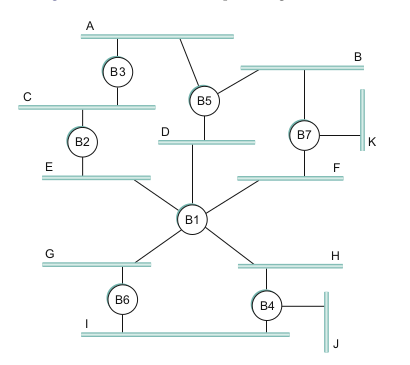
\includegraphics[width=0.5\textwidth
]{images/looped-network.png}
	\caption[Red con un ciclo]{Red con un ciclo}
	\label{fig:looped-network}
\end{figure}

Este problema se resuelve haciendo que los bridges ejecuten un algoritmo de \textbf{spaning tree} distribuido. Se piensa en la LAN extendida como si estuviera representada por un grafo que posiblemente tenga ciclos. Un spanning tree es un subgrafo de este grafo que cubre todos los vértices de la red pero no contiene ciclos. Es decir, un spanning tree mantiene todos los vértices del grafo original pero descarta algunas de las aristas.

El siguiente protocolo es utilizado por un conjunto de bridges para acordar el spanning tree para una LAN extendida en particular y funciona de la siguiente manera: Cada bridge tiene un identificador único; para nuestros propósitos, usamos las etiquetas \(B_1\), \(B_2\), \(B_3\), y así sucesivamente.

Los bridges tienen que intercambiar mensajes de configuración entre sí y luego decidir si son el root o un bridge designado en base a estos mensajes. Específicamente, estos mensajes contienen tres piezas de información:
\begin{enumerate}
  \item El ID del bridge que está enviando el mensaje
  \item El ID del bridge que es considerado el root (hasta el momento)
  \item La distancia, medida en saltos (hops), desde el bridge que envía hasta el root
\end{enumerate}

Inicialmente, cada bridge piensa que es la raíz, y por lo tanto envía un mensaje en cada uno de sus puertos identificándose como la raíz y dando una distancia de 0. 

Al recibir un mensaje sobre un puerto en particular, el bridge verifica si ese nuevo mensaje es mejor que el ya almacenado para ese puerto. Éste se considera mejor que la información actualmente grabada si se cumple alguna de las siguientes condiciones:
\begin{itemize}
  \item Identifica una raíz con un ID más pequeño.
  \item Identifica una raíz con un ID igual pero con una distancia más corta.
  \item El ID de la raíz y la distancia son iguales, pero el bridge que envía tiene un ID más pequeño.
\end{itemize}

Si el nuevo mensaje es mejor que la información actualmente grabada, el bridge descarta la información antigua y guarda la nueva. Sin embargo, primero agrega 1 a la distancia ya que el bridge está a un salto más lejos de la raíz que el bridge que envió el mensaje.

Cuando un bridge recibe un mensaje que indica que no es el bridge raíz, es decir, un mensaje de un bridge con un ID más pequeño, el mismo deja de generar mensajes por su cuenta y en su lugar solo reenvía los de otros bridges, después de agregar 1 al campo de distancia. Del mismo modo, cuando un bridge recibe un mensaje que indica que no es el bridge designado para ese puerto, el bridge deja de generara mensajes sobre ese puerto. Por lo tanto, cuando el sistema se estabiliza, solo el bridge raíz sigue generando mensajes, y los otros bridges están reenviando estos mensajes solo sobre los puertos para los que son el bridge designado. En este punto, se ha construido un spanning tree, y todos los bridges están de acuerdo en qué puertos se utilizan en el mismo. Solo esos puertos pueden usarse para reenviar paquetes de datos en la LAN extendida.

En cierto sentido, es eliminando puertos de la topología que la LAN extendida se reduce a un árbol acíclico. Incluso es posible que un bridge no participe en el reenvío de frames, lo que parece un poco extraño a primera vista. Sin embargo, el algoritmo es dinámico, lo que significa que los bridges siempre están preparados para reconfigurarse en un nuevo spanning tree si algún bridge falla, y por lo tanto, esos puertos y bridges no utilizados proporcionan la capacidad redundante necesaria para recuperarse de fallas.

Una cosa importante a tener en cuenta es que, aunque el algoritmo es capaz de reconfigurar el árbol de expansión cada vez que falla un bridge, no es capaz de reenviar frames por rutas alternativas para evitar un bridge congestionado.

Dado que el objetivo de un bridge es extender una LAN de manera transparente a través de múltiples redes, y dado que la mayoría de las LAN admiten tanto broadcast como multicast, los bridges también deben admitir estas dos características. Broadcast es simple: cada bridge reenvía un frame con una dirección de destino de broadcast en cada puerto activo que no sea el puerto por el que se recibió el frame.

Multicast se puede implementar de la misma manera, con cada host decidiendo por sí mismo si aceptar o no el mensaje.


El algoritmo del árbol de expansión se puede extender para podar las redes sobre las cuales no es necesario reenviar los frames multicast. Cada host que es miembro del grupo M debe periódicamente enviar un frame con la dirección para el grupo M en el campo de origen del encabezado del frame. Este frame tendría como dirección de destino la dirección multicast para los bridges. Sin embargo, esto es ineficiente, por lo que en general se usa la primera opción.

\subsubsection{Limitaciones de los bridges}
En cuanto a la escala, no es realista conectar más de unas pocas LAN mediante bridges. Una razón para esto es que el algoritmo del spanning tree escala linealmente. Una segunda razón es que los bridges reenvían todos los frames de broadcast.

Un enfoque para aumentar la escalabilidad de las LAN extendidas es la VLAN. Las VLAN permiten que una sola LAN extendida se divida en varias LAN separadas. A cada LAN virtual se le asigna un identificador (a veces llamado color), y los paquetes solo pueden viajar de un segmento a otro si ambos segmentos tienen el mismo identificador. Esto tiene el efecto de limitar el número de segmentos en una LAN extendida que recibirá cualquier paquete de broadcast.

En cuanto a la heterogeneidad, los bridges son bastante limitados en los tipos de redes que pueden interconectar. En particular, los bridges utilizan el header del frame de la red y, por lo tanto, solo pueden admitir redes que tengan exactamente el mismo formato para las direcciones. Por lo tanto, los bridges se pueden usar para conectar Ethernets a Ethernets, anillos de tokens a anillos de tokens y una red 802.11 a otra. También es posible poner un bridge entre, por ejemplo, un Ethernet y una red 802.11, ya que ambas redes admiten el mismo formato de dirección de 48 bits. Sin embargo, los bridges no se generalizan fácilmente a otros tipos de redes con diferentes formatos de direccionamiento.